\documentclass[10pt,twocolumn]{article}
\usepackage[margin=0.75in,columnsep=0.25in]{geometry}
\usepackage{times}
\usepackage{amsmath,amssymb}
\usepackage{graphicx}
\usepackage{booktabs}
\usepackage{caption}
\usepackage{hyperref}
\usepackage{authblk}
\usepackage[T1]{fontenc}
\usepackage{titlesec}
\usepackage{abstract}

\hypersetup{colorlinks=true, linkcolor=blue, citecolor=blue, urlcolor=blue}
\captionsetup{font=small, labelfont=bf}
\titlespacing*{\section}{0pt}{10pt}{6pt}
\titlespacing*{\subsection}{0pt}{8pt}{4pt}
\renewcommand{\Authfont}{\normalsize}
\renewcommand{\Affilfont}{\small\itshape}

\title{\Large\bfseries CommerceCore: A Small, Self-Hosted Language Model for Ecommerce Query Constraint Extraction and Entity Segmentation}

\author{Arghya Mukherjee}
\affil{Independent Researcher \\ \texttt{arghya@lightnexus.ai}}
\date{}

\begin{document}
\maketitle

\begin{abstract}
Ecommerce search systems must convert free-text shopping queries into structured constraints that a catalog can act on. We show that a small, openly-licensed language model (Qwen3-1.7B), fine-tuned via QLoRA on a mixture of real human-annotated data and mechanically-validated synthetic data, matches or exceeds several frontier language models (Claude Haiku 4.5, Claude Sonnet 5, GPT-6-tier cheap and flagship variants) on this task, at a training cost under one dollar and a total project cost under ten dollars. On the public QueryNER entity-segmentation benchmark (993 held-out examples), our fine-tuned model achieves F1 = 0.498 (95\% CI: [0.475, 0.523], 10,000-resample bootstrap), compared to 0.204--0.427 for the frontier models we tested. On a held-out constraint-extraction set, our model achieves F1 = 0.683 across three verticals (fashion, grocery, general merchandise), compared to 0.504--0.618 for the same frontier baselines. We report these results alongside a second, independent evaluation on six deliberately harder queries (involving negation, unit conversion, and dense multi-constraint phrasing) on which our model does \emph{not} lead --- Claude Sonnet 5 (F1 = 0.493) and a cheap-tier GPT model (F1 = 0.428) both outperform our model (F1 = 0.400) in this harder regime. We further show that self-hosting is not automatically cheaper than a cheap API tier at low request volume: at our measured single-request throughput, self-hosted serving costs \$0.000116--\$0.000210 per query, versus \$0.000033 for a cheap-tier GPT baseline. We present these results not as weaknesses to conceal but as evidence that our headline claims are real but scope-limited, and we analyze the specific failure modes that a small amount of training data with narrow templated coverage produces. We disclose that a closely related approach was published concurrently with this work, and we position our contribution specifically: a multitask formulation combining constraint extraction and entity segmentation, trained on a mixture of real and mechanically-gated synthetic data, with an explicit and reproducible model-selection procedure based on measured retention against catastrophic forgetting. All code, data, training logs, and the trained model are publicly released.
\end{abstract}

\section{Introduction}

Ecommerce search boxes receive queries such as \emph{``black waterproof trainers under 80 pounds''} or \emph{``almonds with no added sugar.''} To act on such a query --- to filter a catalog, rank candidate products, or explain why a result was returned --- a system needs a structured representation of what the shopper actually specified: a set of (field, operator, value) constraints, or, at a lower level, a segmentation of the query into typed entity spans.

It is tempting to assume that a frontier large language model (LLM), given a reasonable prompt, solves this problem by default. We show this assumption does not hold reliably, and we argue the reasons are structural rather than incidental to prompt engineering:

\begin{enumerate}
\item \textbf{Task narrowness versus model breadth.} Frontier LLMs are trained and evaluated on broad distributions --- open-domain question answering, multi-step reasoning, code generation, dialogue. A narrow, repetitive schema-extraction task over an ecommerce-specific field vocabulary (e.g., \texttt{price\_gbp}, \texttt{contains\_added\_sugar}, \texttt{warranty\_months}) does not exercise the capabilities these models are optimized for.
\item \textbf{Cost and latency at production scale.} A live, search-as-you-type interface requires sub-second response times on every keystroke, at a request volume that can reach millions of queries per day.
\item \textbf{Data locality.} A self-hosted small model keeps customer search and purchase data inside the operator's own infrastructure, a concrete requirement in privacy-sensitive verticals.
\end{enumerate}

We test the ``frontier models solve this by default'' assumption directly rather than assuming it. On a held-out constraint-extraction set and on the public QueryNER benchmark, we measure four frontier systems and find F1 scores in the range 0.20--0.62. We then fine-tune a 1.7-billion-parameter open-weight model (Qwen3-1.7B, Apache-2.0 license) via quantized low-rank adaptation (QLoRA), and show that the fine-tuned model exceeds every tested frontier baseline on both evaluation sets, at a measured training cost of \$0.90 and a total project cost under ten dollars.

Critically, we do not stop at the favorable result. We construct a second, independent evaluation set of six queries specifically designed to probe harder linguistic phenomena --- negation, non-standard unit conversion, and four-or-more-constraint compositionality. On this harder set, our model's advantage disappears: two of the four frontier baselines outperform it. We report this honestly and analyze the failure modes directly from model output.

Our contributions are:

\begin{enumerate}
\item A multitask fine-tuning approach that trains constraint extraction and entity segmentation jointly on a single small model, using a training mixture that combines real human-annotated data (QueryNER) with synthetic data generated under an explicit label-integrity constraint (\S\ref{sec:method}).
\item A checkpoint-selection procedure that measures task performance and retention jointly at every evaluation point (\S\ref{sec:method}).
\item An honest, two-part evaluation: a primary benchmark on which our model leads, and a secondary, harder benchmark on which it does not (\S\ref{sec:results}).
\item A fully reproducible, publicly released artifact: model weights, training data, code, and complete logs (\S\ref{sec:repro}).
\end{enumerate}

We disclose in \S\ref{sec:related} that a closely related approach was published concurrently with the development of this work, and we position our specific contribution relative to it.

\section{Background and Related Work}
\label{sec:related}

\subsection{Small Language Models for Domain Specialization}
A growing body of work argues that task-specific fine-tuning of small language models can match or exceed general-purpose frontier models on narrow tasks. Closest to our work, Licardo and Tankovic \cite{licardo2025} fine-tune a 1-billion-parameter Llama 3.2 model via QLoRA on synthetically generated ecommerce intent-recognition data, reporting approximately 99\% accuracy. We adopt a broadly similar strategy but differ in task formulation (multi-field constraint extraction and entity segmentation, rather than single-label intent classification), base model, and training data composition (real \emph{and} synthetic data, rather than fully synthetic). We do not claim novelty for the general strategy of small-model-plus-QLoRA-plus-synthetic-data.

\subsection{Multitask Ecommerce Language Models}
Li et al.\ \cite{li2023ecomgpt} instruction-tune a large language model across multiple ecommerce subtasks via a chain-of-task formulation. Our work shares the multitask framing but operates at a substantially smaller parameter budget and narrower task scope; we do not perform an independent re-benchmark against this line of work.

\subsection{Synthetic Data Quality for LLM Post-Training}
A recognized challenge in LLM post-training is that synthetic data can be internally consistent while failing a real quality bar not captured by any single automated check. General frameworks such as CuratorKIT \cite{curatorkit2026} implement multiple complementary quality gates for this problem. We implement a narrower, task-specific instance: we find, by manual inspection, that 70\% of an early synthetic batch used a generic, repetitive query template despite passing every mechanical validation check we had implemented.

\subsection{Catastrophic Forgetting in Fine-Tuning}
Parameter-efficient fine-tuning methods such as LoRA do not, by construction, guarantee retention of a base model's general capabilities; empirical measurement is required. We measure retention directly at every checkpoint using a fixed set of task-unrelated probes.

\section{Methodology}
\label{sec:method}

\subsection{Task Definition and Dataset Composition}
We define two tasks, trained jointly: \textbf{constraint extraction} (query $\rightarrow$ list of (field, operator, value) triples) and \textbf{entity segmentation} (query $\rightarrow$ labeled spans, following the QueryNER schema).

\begin{table}[h]
\centering
\small
\caption{Training data sources and provenance.}
\label{tab:data}
\begin{tabular}{lrl}
\toprule
Source & N & License \\
\midrule
QueryNER (sampled) & 1{,}500 & CC BY 4.0 \\
Synthetic query-constraint & 450 & Generated \\
Synthetic catalog-attribute & 180 & Generated \\
\bottomrule
\end{tabular}
\end{table}

For synthetic query-constraint examples, we use a \textbf{structured-scenario-first} procedure: we (1) deterministically sample a product scenario and fixed constraint labels in code, with no LLM involvement, then (2) issue a single LLM call whose only task is to paraphrase the fixed scenario into natural language, never to decide what the constraints are. A downstream mechanical validator confirms each constraint's value is a literal substring of the paraphrase; unmatched constraints are dropped rather than retained with a fabricated evidence span.

\subsubsection{Data Quality Gates}
We implement four mechanical checks: (1) \emph{schema validity}, (2) \emph{source-span binding}, (3) \emph{execution correctness} against a synthetic catalog simulator, and (4) \emph{naturalness} --- a check added after finding, by manual inspection, that 313 of 450 examples (69.6\%) in an early batch used a generic ``products with X'' template despite passing checks (1)--(3). We regenerated the training data after adding this check.

\subsection{Models and Baselines}
\textbf{Fine-tuned model:} Qwen3-1.7B (Apache-2.0), QLoRA with 4-bit NF4 double quantization, bfloat16 compute, LoRA rank 16, alpha 32, dropout 0.05. \textbf{Frontier baselines}, cheap and flagship tier, few-shot prompted: Claude Haiku 4.5, Claude Sonnet 5, a cheap-tier GPT model, and a flagship reasoning GPT model. \textbf{Open-weight baselines} (unfine-tuned): Qwen3.5-2B and SmolLM3-3B \cite{smollm3}, both Apache-2.0.

\begin{figure}[t]
\centering
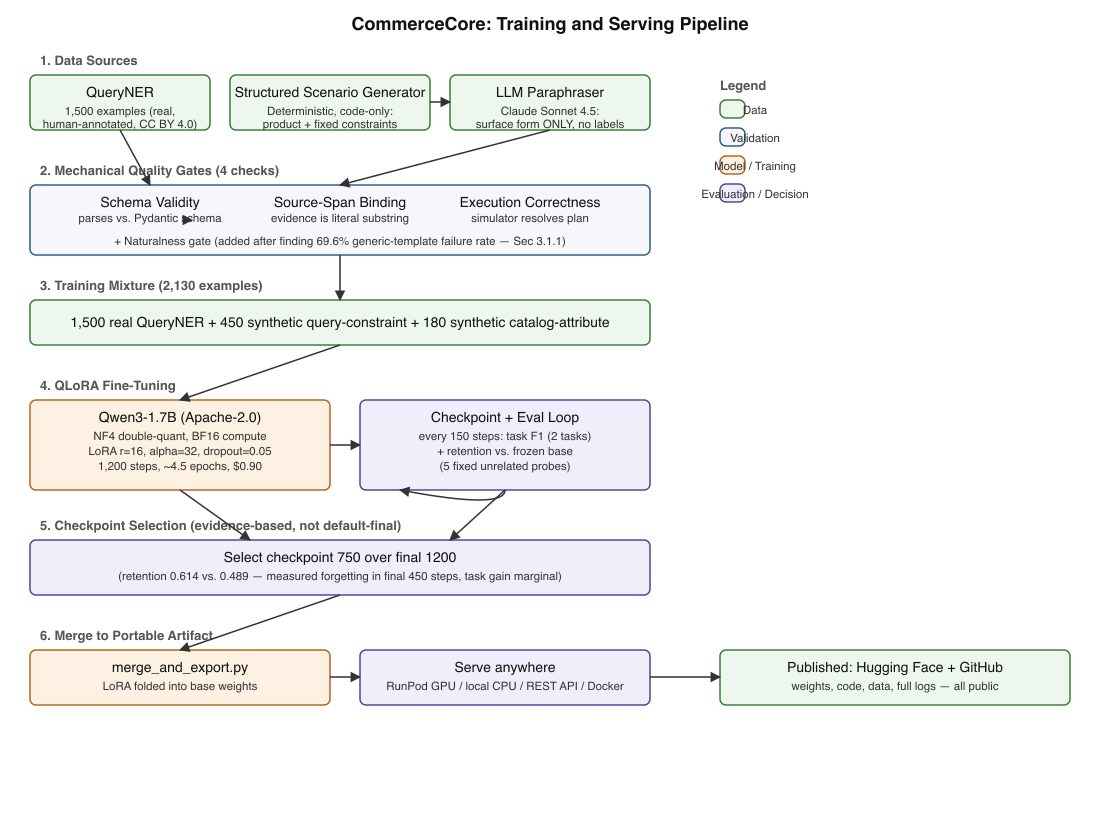
\includegraphics[width=\columnwidth]{architecture_diagram.png}
\caption{CommerceCore training and serving pipeline: data sources, mechanical quality gates, QLoRA fine-tuning with per-checkpoint evaluation, evidence-based checkpoint selection, and public release.}
\label{fig:pipeline}
\end{figure}

\subsection{Experimental Pipeline}
\textbf{Fine-tuning.} Training ran 1,200 optimizer steps (microbatch 1, gradient accumulation 8, $\approx$4.5 epochs over 2,130 examples) on one RunPod RTX PRO 4500 GPU (32GB). Peak VRAM: 2.13GB. Total time: 75.2 minutes; cost: \$0.90.

We checkpoint every 150 steps, evaluating: (a) constraint-extraction F1, (b) QueryNER F1, and (c) retention --- mean token-overlap similarity between the current checkpoint's output and the frozen base model's output on 5 fixed, task-unrelated probes.

\textbf{Checkpoint selection.} We observed retention scores of 0.597, 0.611, 0.597, 0.592, 0.614, 0.490, 0.518, and 0.489 at checkpoints 150--1,200. Retention declines measurably over the final three checkpoints without recovering, while task F1 improves only marginally. We select checkpoint 750 (constraint F1 0.725, QueryNER F1 0.556, retention 0.614) over the final checkpoint 1,200 (constraint F1 0.740, QueryNER F1 0.530, retention 0.489).

\subsection{Evaluation Framework}
We evaluate on the full QueryNER test set (993 examples, CC BY 4.0), reporting a 95\% CI via 10,000-resample bootstrap, and a held-out constraint-extraction set (20 examples, tagged by vertical). We additionally construct a secondary, adversarially-harder set of six queries (negation, unit conversion, 4+ constraint compositionality), reported separately.

\section{Results}
\label{sec:results}

\subsection{Primary Benchmark: QueryNER (Full Test Set)}
\begin{table}[h]
\centering
\small
\caption{Entity segmentation F1, full 993-example QueryNER test set.}
\begin{tabular}{lr}
\toprule
System & F1 \\
\midrule
GPT flagship (reasoning) & 0.204 \\
Claude Haiku 4.5 & 0.263 \\
GPT cheap tier & 0.294 \\
Claude Sonnet 5 & 0.427 \\
\textbf{CommerceCore (ours)} & \textbf{0.498} [0.475, 0.523] \\
\bottomrule
\end{tabular}
\end{table}

Our model exceeds every tested frontier configuration, with a 95\% CI that does not overlap the next-best baseline.

\subsection{Primary Benchmark: Constraint Extraction}
\begin{table}[h]
\centering
\small
\caption{Constraint-extraction F1, held-out set (20 examples).}
\begin{tabular}{lr}
\toprule
System & F1 \\
\midrule
GPT flagship (reasoning) & 0.504 \\
Claude Haiku 4.5 & 0.518 \\
Claude Sonnet 5 & 0.592 \\
GPT cheap tier & 0.618 \\
\textbf{CommerceCore (ours)} & \textbf{0.683} \\
\bottomrule
\end{tabular}
\end{table}

Per-vertical: fashion 0.690, grocery 0.667, general 0.694.

\subsection{Open-Weight Model Comparison}
\begin{table}[h]
\centering
\small
\caption{Unfine-tuned open-weight models, few-shot.}
\begin{tabular}{lrrr}
\toprule
Model & Params & F1 (held) & F1 (\S\ref{sec:secondary}) \\
\midrule
Qwen3.5-2B & 2B & 0.05 & 0.00 \\
SmolLM3-3B & 3B & 0.10 & 0.00 \\
\bottomrule
\end{tabular}
\end{table}

Both are larger than our 1.7B model and score far below it, indicating the gain is attributable to fine-tuning, not scale.

\subsection{Secondary Evaluation: Adversarially-Constructed Queries}
\label{sec:secondary}
\begin{table}[h]
\centering
\small
\caption{F1 on six deliberately harder, independent queries.}
\begin{tabular}{lr}
\toprule
System & F1 \\
\midrule
GPT flagship (reasoning) & 0.167 \\
Qwen3.5-2B (unfine-tuned) & 0.000 \\
SmolLM3-3B (unfine-tuned) & 0.000 \\
Claude Haiku 4.5 & 0.298 \\
\textbf{CommerceCore (ours)} & 0.400 \\
GPT cheap tier & 0.428 \\
Claude Sonnet 5 & 0.493 \\
\bottomrule
\end{tabular}
\end{table}

On this harder set, our model does not lead. Direct inspection identifies three failure patterns: (1) \textbf{multi-constraint recall degradation} on 4+-constraint queries; (2) \textbf{unit/vocabulary normalization failure} (e.g. ``3 year'' not converted to 36 months); (3) \textbf{negation mishandling} (e.g. ``not black'' kept as a literal value).

\section{Discussion}

\subsection{A Small Model Can Beat Frontier Models, Within a Bounded Regime}
Our primary result is consistent with, and independently reproduces at a different task, a finding also reported concurrently \cite{licardo2025}. We consider the explicit characterization of the \emph{boundary} of this result (\S\ref{sec:secondary}) more informative than the headline comparison alone.

\subsection{Serving Cost: Not Automatically Cheaper Than a Cheap API Tier}
At our measured throughput (3,429--6,207 queries/hour on one GPU), self-hosted serving costs \$0.000116--\$0.000210 per query. For a representative request (100 in / 30 out tokens), frontier costs range from \$0.000033 (GPT cheap tier) to \$0.000950 (GPT-5 flagship). We disclose that an earlier draft of this analysis incorrectly concluded self-hosting was cheaper; we caught and corrected this. Self-hosting overtakes GPT's cheap tier on cost only past $\approx$21{,}800 queries/hour --- achievable via batching, which we did not measure. The accurate case for self-hosting is data locality and higher accuracy than the cheap-tier baseline, not raw cost at low volume.

\subsection{Retention Measurement Changes Model Selection}
Selecting the final checkpoint by default would have released a model with measurably worse retention (0.489 vs.\ 0.614) for only a marginal task-metric gain.

\subsection{Synthetic Data Passing Mechanical Checks Is Not Sufficient}
69.6\% of an early synthetic batch failed a real quality bar that no automated check we had implemented would have caught.

\subsection{Limitations}
(1) \textbf{Scale}: 2,130 training examples and a 20-example primary held-out set are small. (2) \textbf{Task scope}: only 2 of 4 originally-scoped tasks are fully evaluated. (3) \textbf{Novelty scope}: the general small-model-QLoRA-synthetic-data strategy is not novel to this work. (4) \textbf{Baseline coverage}: two providers, two tiers each, tested. (5) \textbf{Single-run training}: no multi-seed averaging.

\section{Reproducibility}
\label{sec:repro}
We release model weights (\href{https://huggingface.co/arghya2030/commercecore-qwen3-1.7b}{Hugging Face}), source code (\href{https://github.com/arghya05/commercecore}{GitHub}), training data including the QueryNER subsample and both synthetic datasets, full per-step training logs, and full evaluation scripts. Total measured cost for the complete study was under \$10.

\section{Conclusion}
We show that a small, openly-licensed language model, fine-tuned at a cost of under one dollar, can exceed several frontier language models on two narrow ecommerce tasks, evaluated on a real public benchmark and a held-out set. We report this alongside its explicit boundary, an honest serving-cost analysis with a self-caught correction, and a fully reproducible artifact.

\section*{Acknowledgments}
We used Claude (Anthropic) and GPT (OpenAI) models both as evaluation baselines and, in a separate and disclosed role, to assist in synthetic training data generation and manuscript preparation.

\begin{thebibliography}{9}

\bibitem{licardo2025}
J. T. Licardo and N. Tankovic, ``Performance Trade-offs of Optimizing Small Language Models for E-Commerce,'' \emph{arXiv preprint arXiv:2510.21970}, 2025.

\bibitem{li2023ecomgpt}
Y. Li, S. Ma, X. Wang, S. Huang, C. Jiang, H.-T. Zheng, P. Xie, F. Huang, and Y. Jiang, ``EcomGPT: Instruction-tuning Large Language Models with Chain-of-Task Tasks for E-commerce,'' \emph{arXiv preprint arXiv:2308.06966}, 2023.

\bibitem{curatorkit2026}
``CuratorKIT: Data Curation and Synthetic Data Generation for LLM Post-Training,'' \emph{arXiv preprint arXiv:2606.21631}, 2026.

\bibitem{palenmichel2024}
C. Palen-Michel, L. Liang, Z. Wu, and C. Lignos, ``QueryNER: Segmentation of E-commerce Queries,'' in \emph{Proc.\ LREC-COLING 2024}, arXiv:2405.09507.

\bibitem{qwen3}
Qwen Team, Alibaba Group, ``Qwen3 Technical Report,'' \emph{arXiv preprint arXiv:2505.09388}, 2025.

\bibitem{esci}
Amazon Science, ``Shopping Queries Dataset (ESCI): A Large-Scale Dataset for Improving Search Relevance in E-commerce,'' 2022.

\bibitem{smollm3}
Hugging Face TB Research, ``SmolLM3: A Long-Context, Multilingual, Reasoning Small Language Model,'' 2025.

\end{thebibliography}

\end{document}
